% ---------------------------------------------------------------------
%  2  METHODOLOGY
%  Sources: hourly-base-data.ipynb, data-analysis.ipynb,
%           classical-models.ipynb, neural-models.ipynb,
%           timestral-zero-shot.ipynb, Correlation Analyses/
% ---------------------------------------------------------------------
\section{Methodology}
\label{sec:method}

\subsection{Dataset and Source}
\label{sec:data}
The data is the Kaggle ``Bitcoin Historical Data'' set~\cite{kaggle} of
1-minute Bitstamp BTC/USD candles, pinned to one version so that every
run sees the same file, and aggregated to hourly candles (\texttt{Open},
\texttt{High}, \texttt{Low}, \texttt{Close}, \texttt{Volume}). The models
use the 59{,}331 consecutive hours from 1 January 2020 to 8 October 2026.
Auxiliary sources were tested as extra inputs: hourly BTC and ETH candles
with order flow from Binance~\cite{binance}, about 40 macro and market
series from FRED~\cite{fred} and Yahoo Finance, and 281 US release times
(CPI, payrolls, FOMC) from the BLS and Federal Reserve calendars.

\subsection{Preprocessing}
\label{sec:preproc}
Minutes are aggregated to hours without dropping missing rows, so the
hourly grid stays continuous. The minute data hides gaps: a minute without
trades appears as a flat, zero-volume candle at the previous close. Such
minutes make up 95\% of 2012 and 25--40\% of 2013--2016, against 1--4\%
per year since 2018, so the base series starts in 2018; the models use it
from 2020 so that the training block is closer to the current market.
Outage hours are flagged, not removed; Bitstamp and Binance hourly returns
correlate at 0.993, so the data is clean. Scaling is fitted on training
data only, inside each model pipeline; the LSTM normalises each input
window by itself, and Timestral normalises its own inputs.

\subsection{Exploratory Data Analysis}
\label{sec:eda}
Analyses that could steer a model are fitted on the training block and
checked on validation, never on test. Hourly returns are heavy-tailed
(excess kurtosis 55). Fig.~\ref{fig:acf} shows the central fact of the
project: the autocorrelation of returns is tiny (about $-0.03$ at lags 1,
2 and 24, and with a band that allows for volatility clustering only the
lag-24 reversal stays significant; an AR(24) model has validation
$R^2=-0.002$), while the absolute returns are strongly autocorrelated
(0.30 at lag 1, still 0.10 a week later; an AR(24) on $|\ret|$ explains
10\% of the validation variance). The direction is almost noise; the size
is not.

The size also follows the clock, and this rhythm drifts
(Fig.~\ref{fig:hour}): the 14~UTC peak (US session) rises from 1.28 times
the average hour before the spot ETFs to 1.67 after them, a change that
starts in 2022 and jumps in 2024; weekend hours went from 0.8 to about
0.6 times weekday hours. Volatility regimes persist (the next day moves
0.32\% per hour after calm weeks, 0.71\% after wild ones), but tell how
much Bitcoin will move, not which way. ETH moves with Bitcoin in the same
hour (correlation 0.84) but does not lead it. Macro variables, compared
with Spearman correlations and a false-discovery-rate
correction~\cite{benjamini1995}, follow global risk appetite (S\&P~500:
0.33 daily, 0.53 monthly), but none leads Bitcoin. US releases do move it:
the release hour moves 2.2--2.5 times the same hour on nearby days without
a release (FOMC up to 3.6 times; Wilcoxon $p<0.001$ on train and
validation). From these findings, candidate features (volatility ratios,
minutes without trades, release-hour flags, a 90-day hour profile) were
built, checked for look-ahead and screened on train and validation.

\begin{figure*}[t]
  \centering
  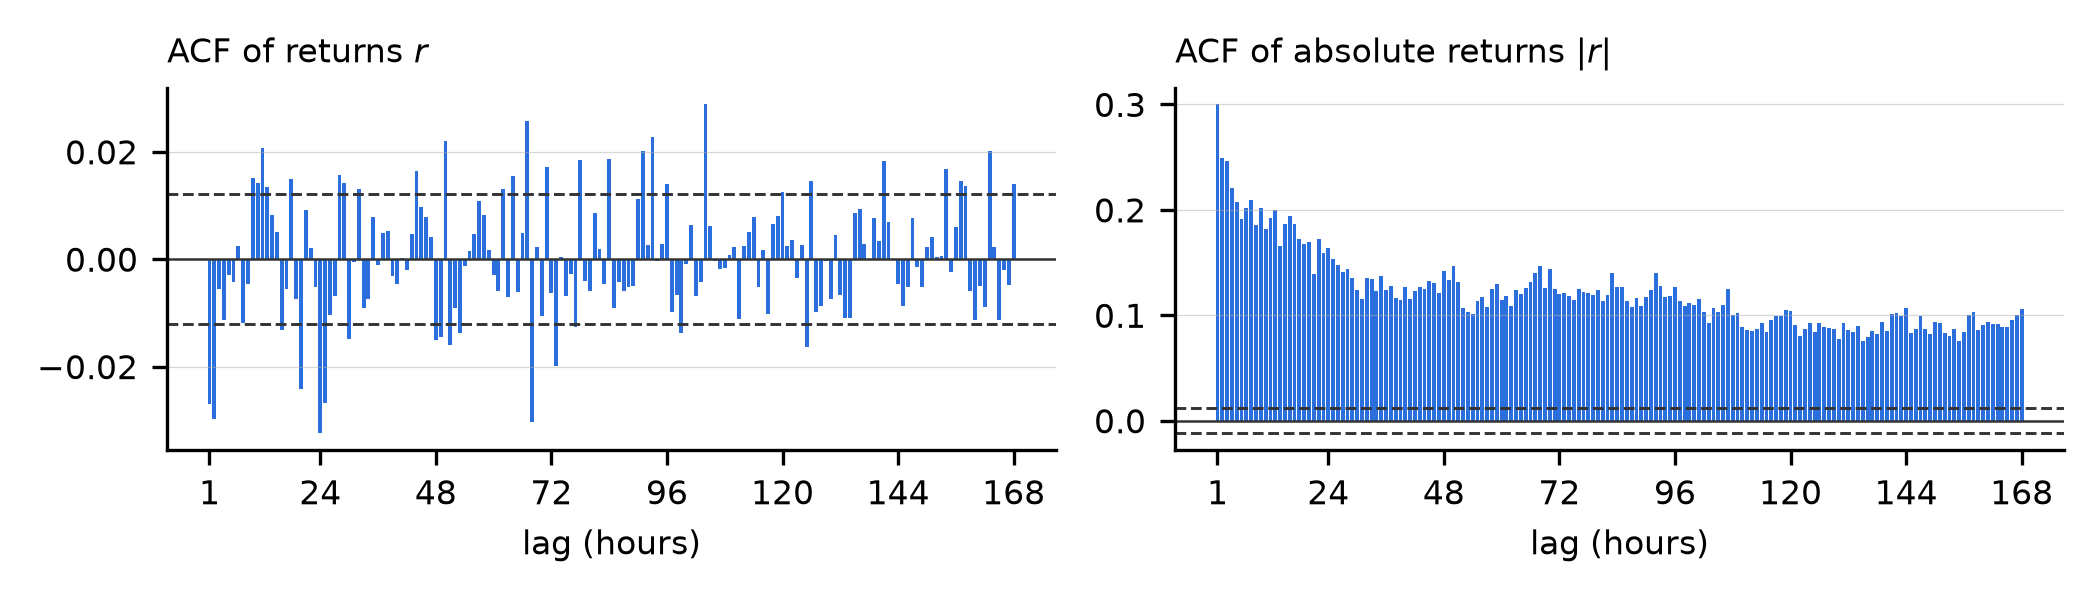
\includegraphics[width=0.78\textwidth]{fig_acf_2020.png}
  \caption{Autocorrelation of hourly returns (left) and of their absolute
  value (right), lags 1--168\,h, training block 2020--2022. Dashed lines:
  95\% band of white noise (too narrow under volatility clustering).}
  \label{fig:acf}
\end{figure*}

\begin{figure}[t]
  \centering
  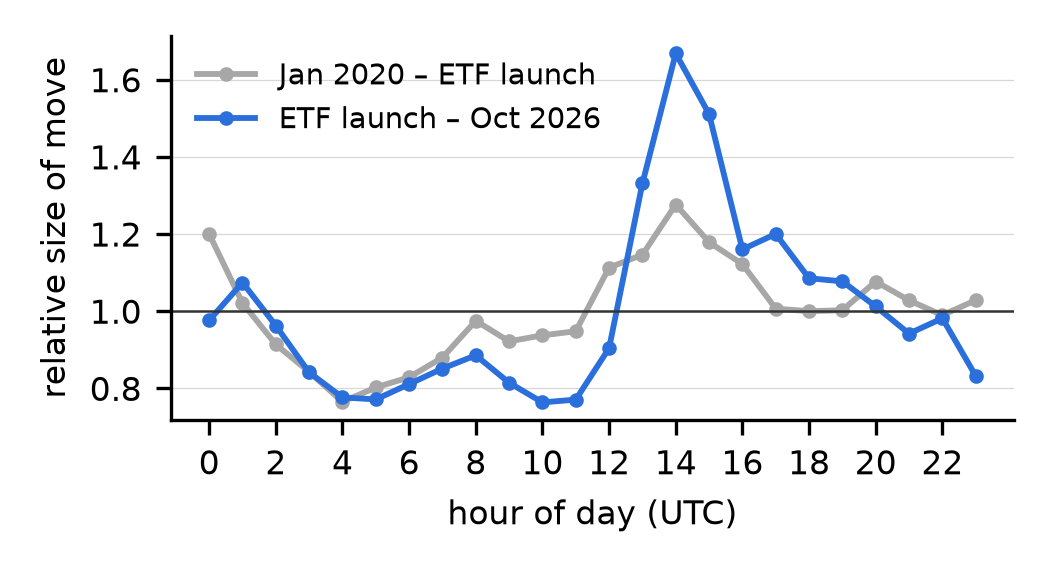
\includegraphics[width=0.9\columnwidth]{fig_hourprofile_2020.png}
  \caption{Size of the hourly move by hour of day (UTC), relative to the
  average hour, before and after the launch of the US spot ETFs
  (11 Jan 2024). The 14~UTC peak already grows from 2022.}
  \label{fig:hour}
\end{figure}

\subsection{Prediction Targets and Features}
\label{sec:targets}
A forecast is made at every hour (the \emph{origin}) that has 30 days of
history before it and 24 target hours after it. Besides the assigned
target, the 24 hourly returns, we ask the questions the data can answer:
(a) the direction of the next hour; (b) the size $|\ret|$ of each of the
next 24 hours; (c) an 80\% prediction range for each of these hours; and
(d) the next day's return, direction and volatility. All features are
scale-free, so they mean the same in 2020 and 2026: lagged returns,
realised volatilities over 24, 72 and 168 hours, high--low ranges, volume
ratios and the calendar (the \emph{base} set). In the \emph{long format}
each origin gives 24 rows, one per predicted hour, with per-hour columns
(the average size of that hour, its size one and seven days earlier). One
model then learns the common structure (``volatile weeks make every hour
volatile'') from 24 times more rows, and the hour-specific part from the
per-hour columns.

\subsection{Models}
\label{sec:models}
\emph{Classical:} Ridge~\cite{hoerl1970}, Lasso~\cite{tibshirani1996},
ElasticNet~\cite{zou2005}, $k$-nearest neighbours, SVR/SVC, Random
Forest~\cite{breiman2001}, Extra Trees~\cite{geurts2006}, Gradient
Boosting (GB)~\cite{friedman2001} and averages of them. Ranges come from
GB with the quantile loss~\cite{koenker1978} for the 10\% and 90\%
quantiles, recalibrated by \emph{rolling conformal
calibration}~\cite{vovk2005,gibbs2021}: the half-width is multiplied by
the factor that would have given 80\% coverage over the last 30 days of
known outcomes; the \emph{Mondrian} variant does this separately for
release hours. Both volatility targets are also refitted every month on
all data known by then: with weights that halve every 12 months for the
hourly size, with an expanding window for next-day volatility (each chosen
on validation). \emph{Neural:} MLPs (scikit-learn, PyTorch) and
LSTMs~\cite{hochreiter1997} reading a 168-hour window of ten
window-normalised channels, trained with MSE or Huber loss. The best LSTM
also receives the clock and release flags of each predicted hour, reads
the hidden states of the whole week weighted by traded volume (an
attention mask), and is fine-tuned every month. \emph{Foundation model:}
Timestral~\cite{timestral} is pretrained by Mistral AI on mostly synthetic
series, reads a long context in patches of 32 hours and returns 21
quantiles of each of the next 24 hours. It is used zero-shot: its weights
never see our data; we only choose, on validation, which series it reads
($\ret$ or $|\ret|$), the context (30--180 days), the covariates and the
model size. Its expected $|\ret|$ is the mean of the forecast
distribution, since $R^2$ rewards the mean, not the median. GARCH(1,1)
\cite{bollerslev1986} is a classical volatility benchmark.
Table~\ref{tab:hyper} lists the chosen settings.

\begin{table}[t]
\centering
\caption{Main models, tuned grids and settings chosen on validation.}
\label{tab:hyper}
\footnotesize
\setlength{\tabcolsep}{3pt}
\begin{tabular}{@{}L{2.2cm}L{5.9cm}@{}}
\toprule
Model (target) & Grid $\rightarrow$ chosen \\
\midrule
Ridge (returns) & $\alpha \in 0.1$--$10^{9}$ $\rightarrow 10^{5}$
  (strong shrinkage: close to the zero forecast) \\
GB (hourly $|\ret|$) & learning rate $\{0.05, 0.1\}$, depth $\{2,3,6\}$
  $\rightarrow$ 0.1, 6 (depth 3--6 within 0.004); 1{,}000 rows per leaf \\
GB (next-day vol.) & $\rightarrow$ learning rate 0.05, depth 2, 200
  trees, 100 rows per leaf \\
Monthly refit & expanding, 24-month window, half-life 6/12 months
  $\rightarrow$ 12 months ($|\ret|$), expanding (daily) \\
LSTM ($|\ret|$) & 2 layers, hidden $\{32,64,128\} \rightarrow 64$,
  dropout 0.2, Adam $10^{-3}$, weight decay $10^{-4}$, 5 seeds \\
MLP ($|\ret|$, long) & hidden (256, 128), weight decay 0.01 \\
Timestral & 28M/209M $\rightarrow$ 28M; series $|\ret|$; 180 days;
  clock, release calendar, range and volume, ETH size, VIX \\
\bottomrule
\end{tabular}
\end{table}

\subsection{Rationale for the Chosen Methods}
\label{sec:rationale}
Simple rules set the bar a model must beat. Regularised linear models
suit a target that is mostly noise; trees capture non-linear effects of
volatility and the clock; networks test whether a sequence model finds
what hand-made features miss; the foundation model tests whether
pretraining can replace fitting on our data. Monthly refits and conformal
calibration answer the drift seen in the analysis.
